% Activate the following line by filling in the right side. If for example the name of the root file is Main.tex, write
% "...root = Main.tex" if the chapter file is in the same directory, and "...root = ../Main.tex" if the chapter is in a subdirectory.
 
%!TEX root =  secondDraft.tex

\chapter[Simulation of Grote Markt]{Simulation of Grote Markt}

In the previous chapter, we have laid out the process from creating a Bayesian Network from a written scenario of a case, and laid out criteria on how to evaluate that network. In this chapter, the method is applied to a simulation of a robbery at the Grote Markt, the main square of Groningen.

By placing agents in a `real' spatial environment, they are constrained by geography in some manner - they cannot see through buildings, and cannot move through them. These affordances result in more interesting behaviours for the agents, and are a first step towards using this approach to less abstracted societal issues.



\section{Scenario}
There are two agents walking around the area of Grote Markt. One of the agents is old and carries a valuable object. The other agent is young, and might potentially steal the object. If the potential thief sees the potential victim, it decides whether the potential victim is vulnerable enough to steal from, and the object is valuable enough. If both of these conditions are fulfilled, the agent becomes a potential thief, and now has a motive to steal from the old agent. The agent will attempt to sneak up on the victim, and steal the object from the old agent. At some point, the old agent realises that their valuable object is gone. This is the first scenario. In the second scenario, the old agent simply dropped the valuable object, and after a while notices that it is gone. As evidence, we have a psychological report that estimates whether the young agent is capable of the crime, we might have video footage of the thief stealing the object, and we have the fact that the potential thief shows up on camera. 

Additionally, outside the described scenario, we also have access to the `mental' state of the potential thief, so we know whether they actually consider the old agent vulnerable, and whether they find the object itself valuable. We also know if the thief is actually intending to sneak up on the other agent.


\section{Simulation}

We extract the relevant agents from the scenario, we need two of them: a potential thief, and a potential victim. Every agent has an age, to determine whether they are vulnerable or not - old people are considered more vulnerable. Every agent also has an object of a certain value, the thief's object has a value of -1, and the other agent's object has a value of 1000, to make it a tempting target. An agent decides if it wants to steal something by making a very simple risk-calculation based on their risk threshold: if the object is more expensive than their risk threshold, they will attempt to steal it (contributing to `motive'). Every agent also has a goal state, this is the location at the edge of the map. When they enter their goal state, they are essentially removed from the simulation, as they leave the relevant area. Every simulation was run for 100 timesteps, or until both agents are in their goal states. The simulation itself was ran 500 times. The behaviour of the agents is shown in Figure~\ref{behaviourGM}. Agents are placed randomly on the map.

The operationalisation of the random variables is described below. The output node is the node `stealing\_1\_0':
\begin{description}


\item[seen\_1\_0  ] if the victim agent is in the line of sight of the thief agent.
\item[know\_valuable\_1\_0 ] if the value is higher than the risk threshold.
\item[know\_vulnerable\_1\_0  ] if the victim's age is older than the thief's threshold age.
\item[motive\_1\_0 ] if the object is more valuable than the risk threshold, the victim's age is older than the thief's threshold age, and the thief is not already stealing from someone else. 
\item[sneak\_1\_0 ] if the thief has targeted the victim (has a motive) , but is not yet in the same position.
\item[stealing\_1\_0 ] if the thief has targeted the victim, the object's value is greater than the risk threshold, and the thief's position is the same as the victim's position. 
\item[object\_dropped\_accidentally\_0 ] at every epoch, there is a 1/500 probability that the victim agent will drop the object by accident.
\item[E\_vulnerable\_1\_0 ] the thief decides that the target is vulnerable (know\_vulnerable\_1\_0 is true).
\item[E\_valuable\_1\_0 ] the thief decides that the object is valuable (know\_valuable\_1\_0 is true).
\item[E\_sneak\_1\_0 ] the agent sneaks up on the target (sneak\_1\_0 is true).
\item[E\_camera\_1 ] the thief is seen on any one of the cameras.
\item[E\_psych\_report\_1\_0 ] if the thief has a motive, we draw an estimated risk threshold and an estimated age threshold from two normal distributions (mean = victim age, sd = 20), (mean = value good, sd = 100). If the victim is older than the thief's minimal age threshold, and the object more valuable, we estimate that the psych profile states that the victim fits the thief's profile, else not.
\item[E\_camera\_1 ] the thief is seen on any one of the cameras.
\item[E\_object\_gone\_0 ] if the object is dropped accidentally, or if the object has been stolen.
\item[E\_camera\_seen\_stealing\_1\_0 ]  if any camera sees the thief during the state in which it is stealing.
\end{description}

The environment for the agents was created by converting a map image into an agent-readable world. This was done by writing a method to convert screenshots of maps into an agent-readable environment. The maps were screenshotted from \url{http://maps.stamen.com/terrain/#18/53.21618/6.57225} and converted into greyscale. Then, they were transformed into a grid of a given size. The average greyscale value of each cell in the grid was taken and coded as either `accessible' or `non-accessible'. On the greyscale map, the color of the buildings was in the range of (189, 199) - cells within this range were coded as `inaccessible', since agents cannot walk through buildings. All other cells were `accessible'. This resulted in a map shared by all agents that constrained their movements. There are 5 cameras placed randomly on the `accessible' cells on the map, each with a visual radius of 8. Additionally, we used this map to calculate the sight lines of both cameras and agents. An agent or a camera cannot see another agent if there is an `inaccessible' grid cell on the sight line between the two.



\begin{figure}[htbp]
\begin{center}
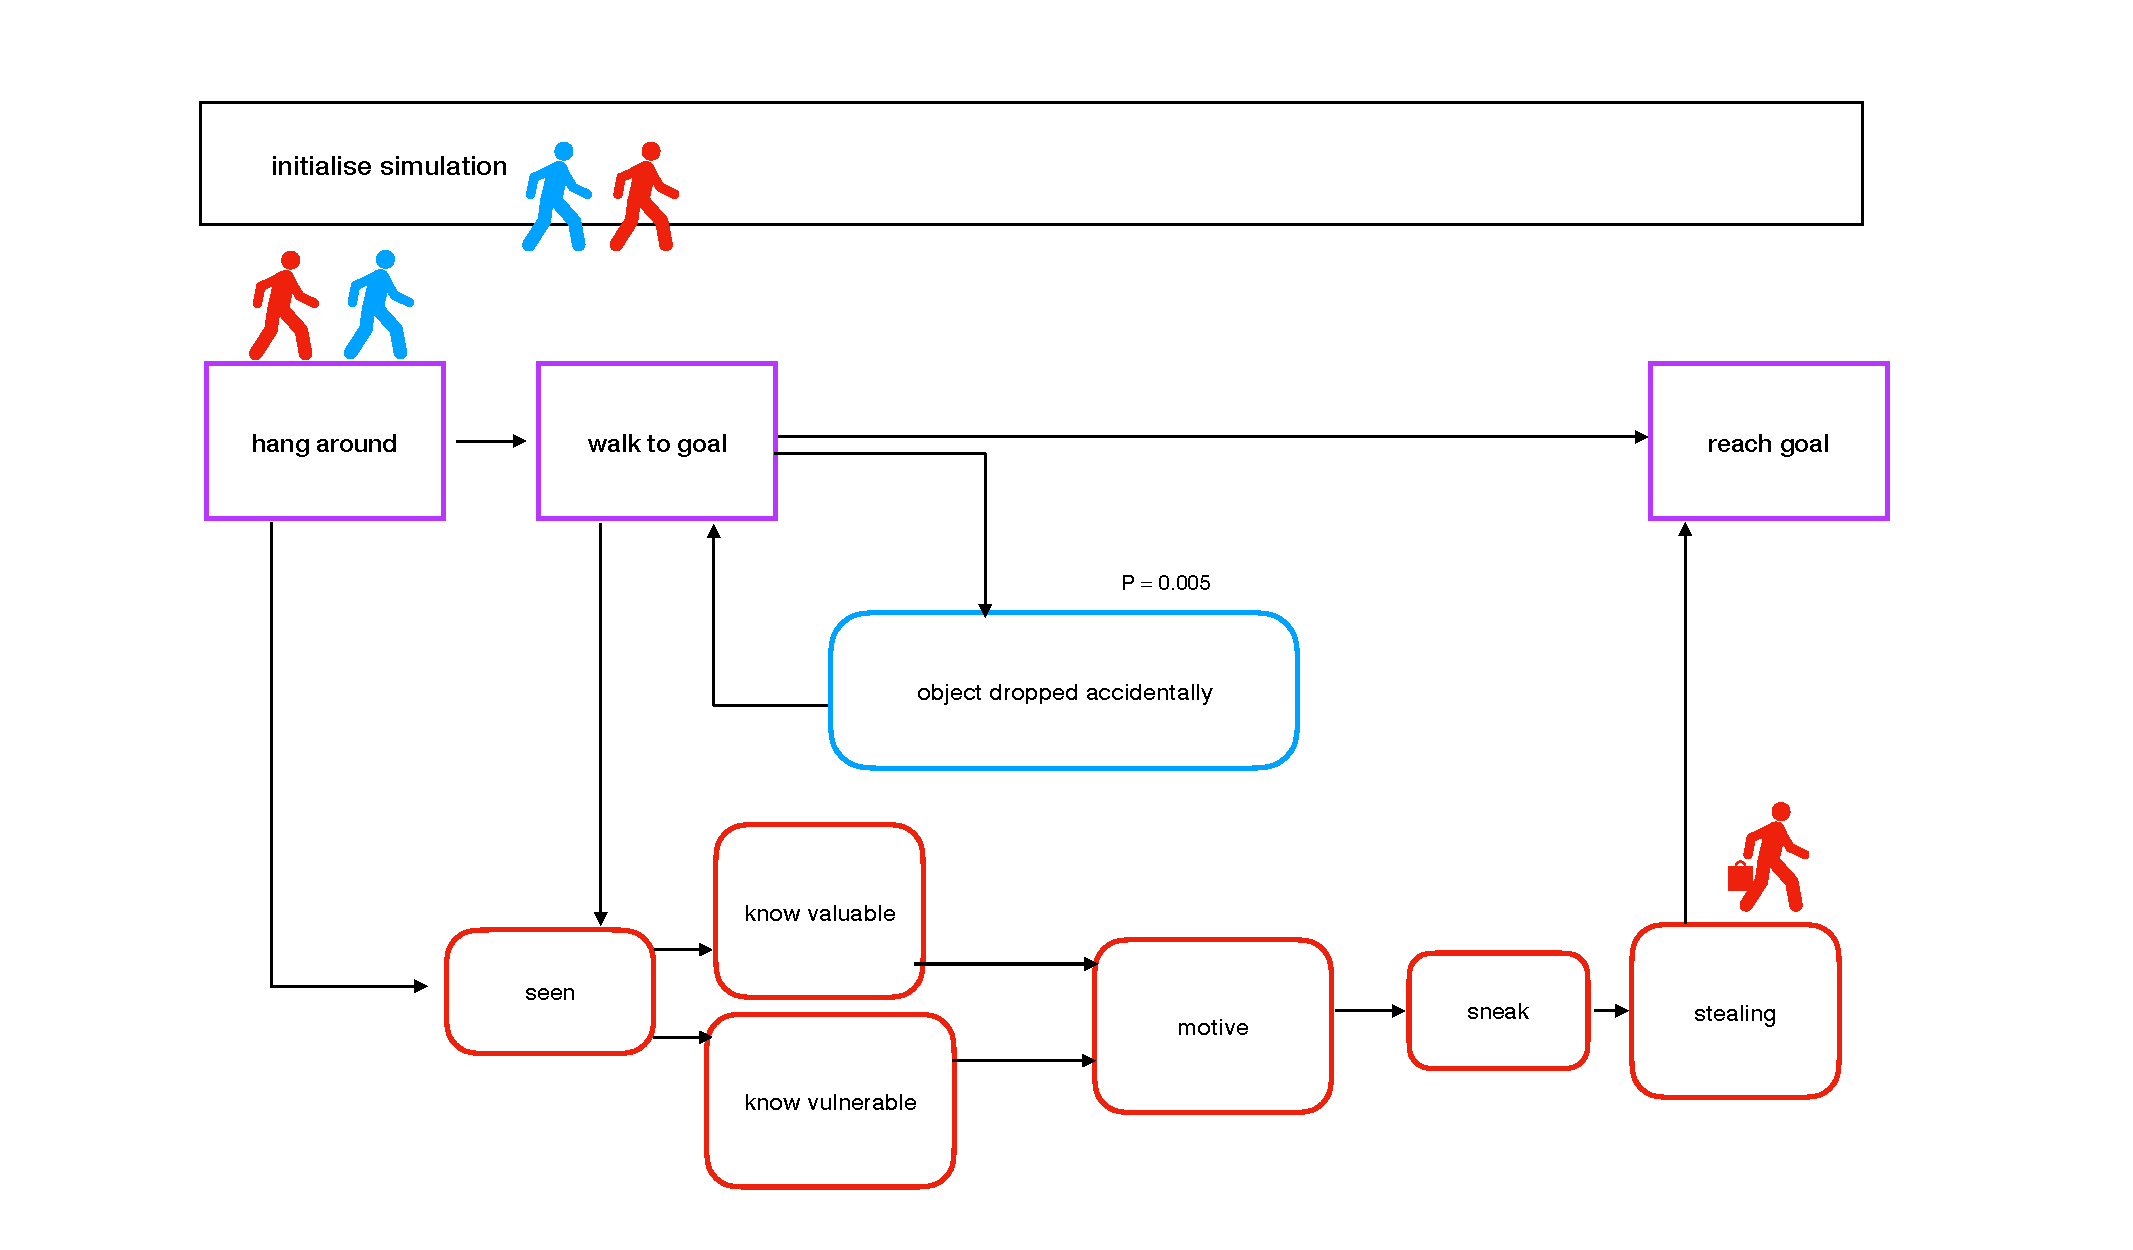
\includegraphics[width=\linewidth]{images/grotemarkt.pdf}
\end{center}
\caption{The behaviour of the agents. The nodes with rounded edges correspond to the nodes in the Bayesian Network.}
\label{behaviourGM}
\end{figure}


\begin{figure}[htbp]
\begin{center}
\begin{subfigure}{.5\textwidth}
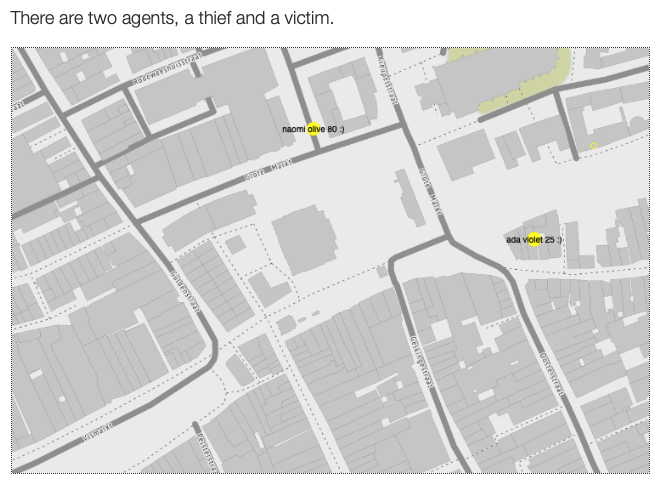
\includegraphics[width=\linewidth]{images/grotemarktmap.png}
\caption{map of environment - 2 agents}
\end{subfigure}%
\begin{subfigure}{.5\textwidth}
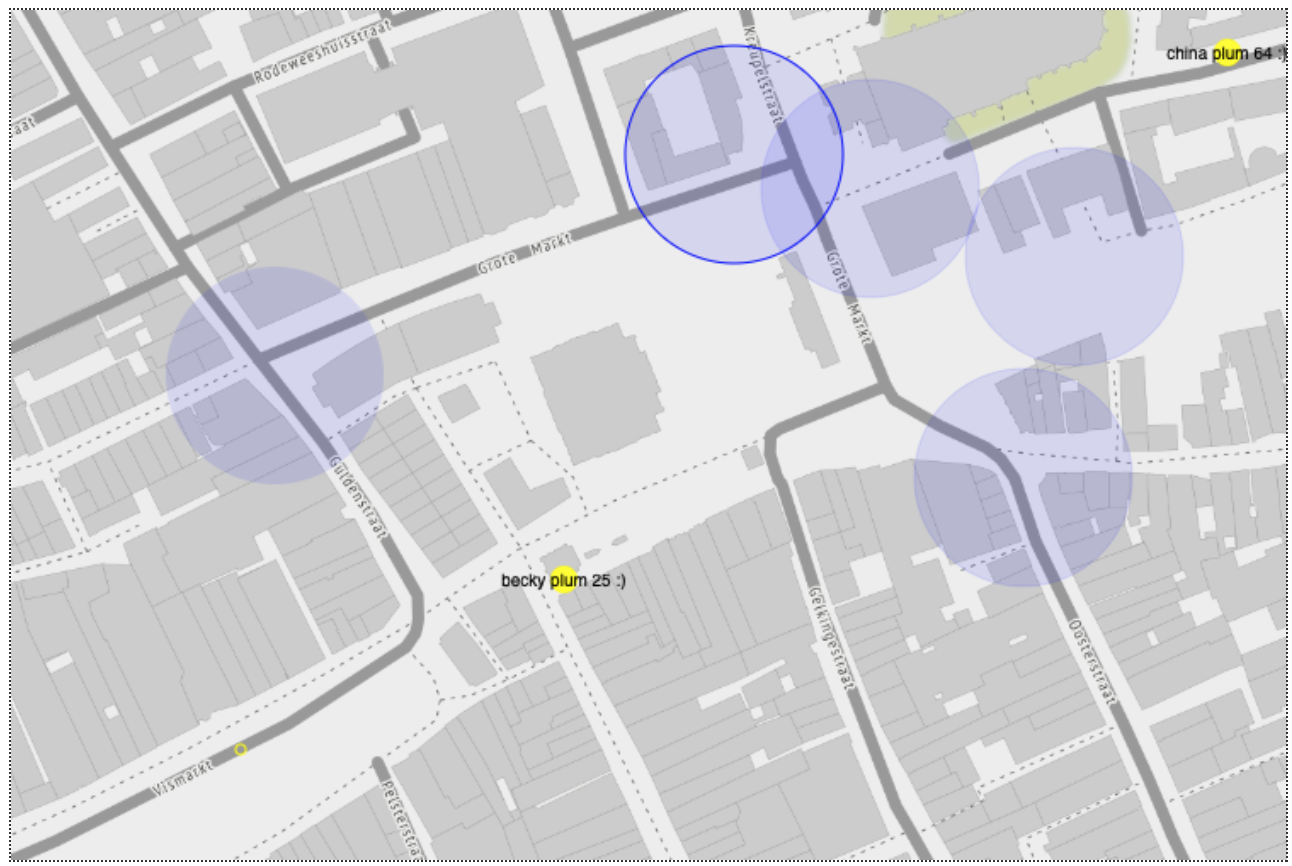
\includegraphics[width=\linewidth]{images/agentGM.png}
\caption{Camera locations are randomly initialized}
\end{subfigure}%
\label{groteMarkt}
\caption{The Grote Markt environment}
\end{center}
\end{figure}





\section{Creating the Bayesian Network}

The network is shown in Figure~\ref{wedding}.

\begin{figure}
\begin{center}
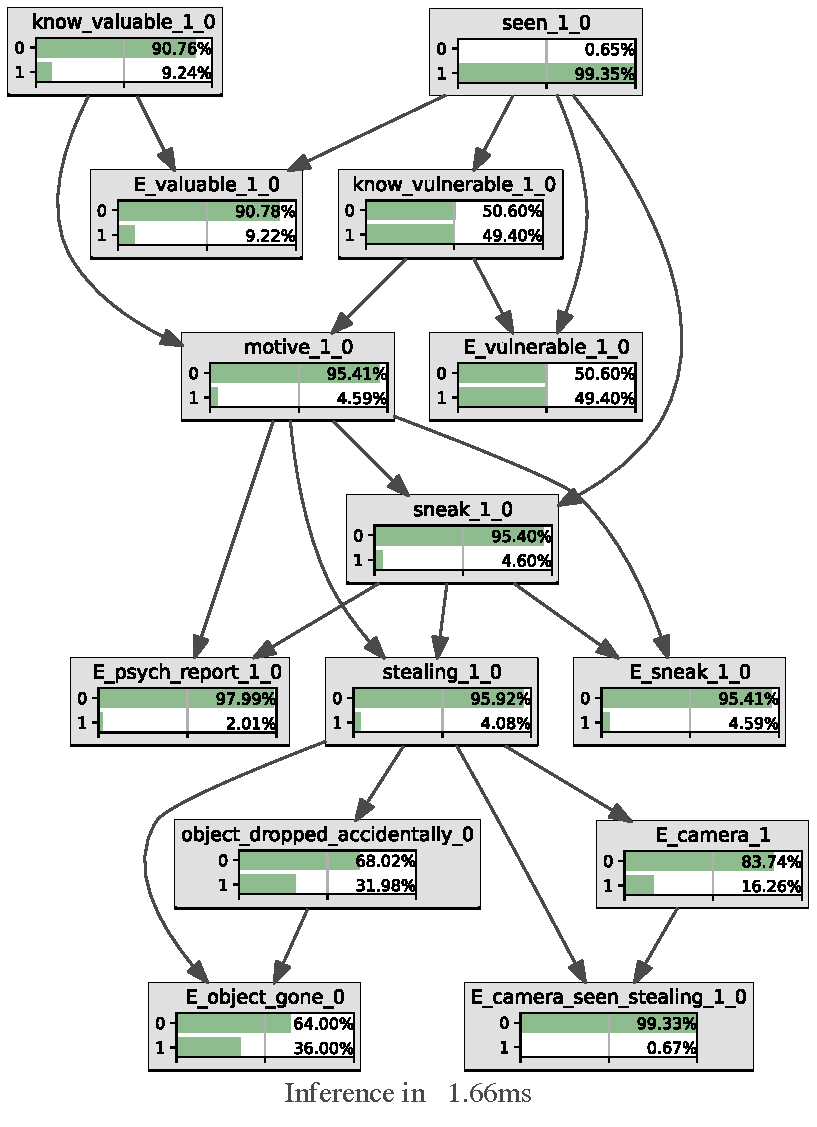
\includegraphics[width=1.2\linewidth]{../experiments/GroteMarkt/bnImage/BNIMAGEGroteMarkt.pdf}
\caption{Network of Grote Markt simulation.}
\label{wedding}
\end{center}
\end{figure}


\section{Evaluation}



\subsection{Numbers}
\begin{enumerate}
\item \textbf{The conditional frequencies in the BN correspond to the conditional frequencies in the simulation}

The frequency of events in the network (without evidence set) correspond to the frequency of events in the simulation within ±0.05, see Table~\ref{testTableGM}.

\begin{table}
\centering
\begin{tabular}{|c|c|c|}
 \hline
 Conclusion & Frequency P(event) & BN P(event)\\
 \hline
seen\_1\_0    & 0.52& 0.52\\
know\_valuable\_1\_0  & 0.046 & 0.469\\
know\_vulnerable\_1\_0  &0.238 &  0.2385\\
motive\_1\_0  & 0.012 &  0.0186\\
sneak\_1\_0  & 0.012& 0.0182\\
stealing\_1\_0  & 0.012 & 0.0177\\
object\_dropped\_accidentally\_0  & 0.186 & 0.187 \\
E\_valuable\_1\_0  & 0.046 &  0.046\\
E\_vulnerable\_1\_0  &0.238 &  0.237\\
E\_psych\_report\_1\_0  & 0.006&  0.002\\
E\_camera\_1 & 0.778 & 0.777\\ 
E\_sneak\_1\_0  & 0.012& 0.018\\
E\_camera\_seen\_stealing\_1\_0  & 0.008 & 0.0116 \\
E\_object\_gone\_0  & 0.198 & 0.197 \\
 \hline
\end{tabular}
\caption{Correspondence}
\label{testTableGM}
\end{table}

\item \textbf{The values in the conditional probability tables are elicitable from human modellers}
(todo)


On the other hand, nodes like `motive' are almost constructed logically (Figure~\ref{cptmotive}), which implies that we might not need to elicit probabilistic information about all hypotheses nodes - if we find appropriate priors for nodes without parents, and their children can be constructed out of logical combinations of their parents, we might only need to elicit probabilistic information for the parents. However, most of the hypothesis nodes are not such logical combinations, and hence need effortful and almost impossible-to-find information about frequencies.

\begin{figure}[htbp]
 \centering
 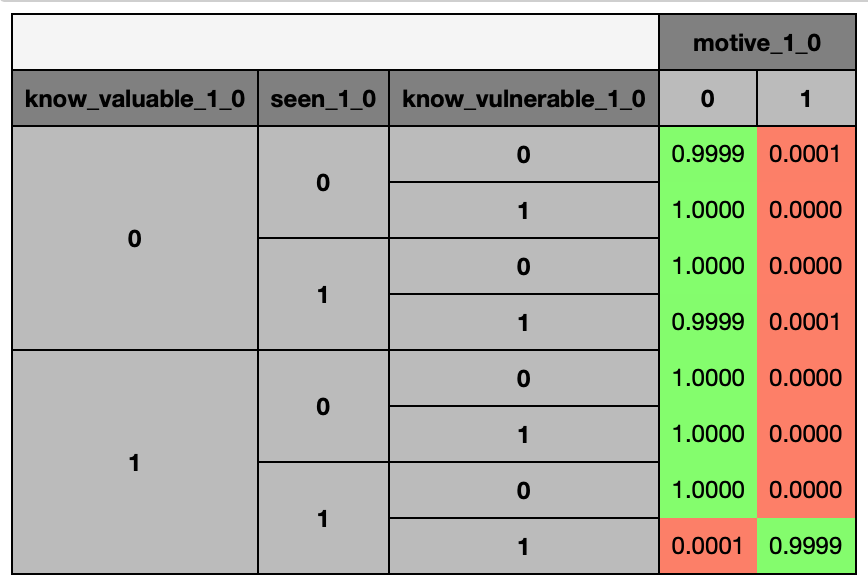
\includegraphics[width=0.6\linewidth]{images/cptMotive.png}
\caption{ Conditional probability table for `motive\_1\_0'. A logical approach.}
\label{cptmotive}
\end{figure}%



\item \textbf{The BN is robust against imprecision in the conditional probability tables}

\begin{figure}[htbp]
\begin{center}
\begin{subfigure}{.5\textwidth}
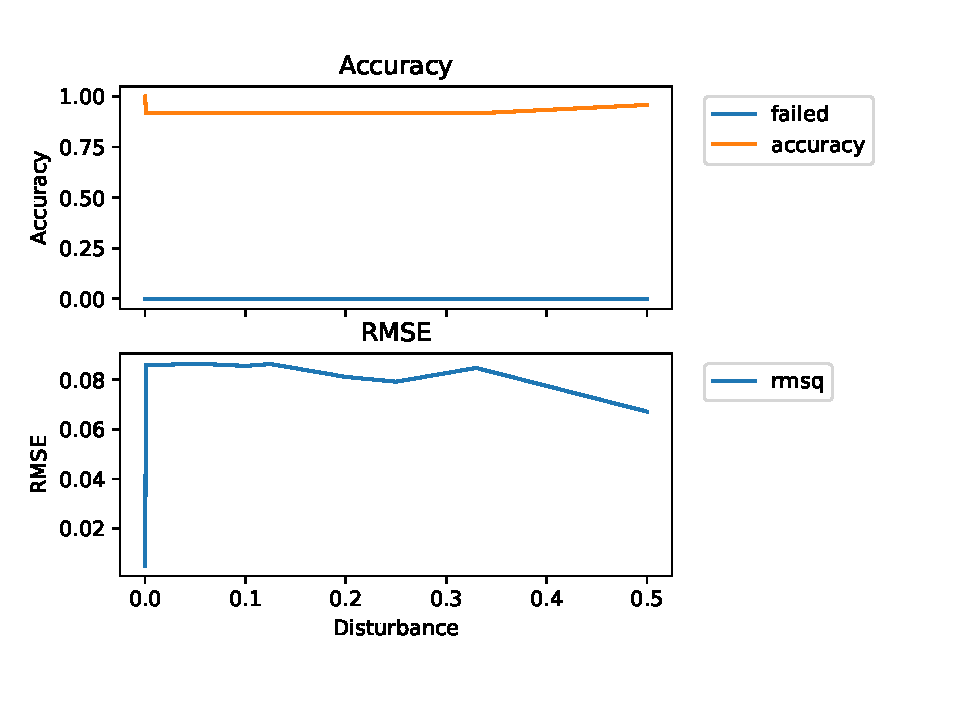
\includegraphics[width=0.9\linewidth]{../experiments/GroteMarkt/plots/performance_GroteMarkt.pdf}
\caption{Network Under Disturbance.}
\label{dist}
\end{subfigure}%
\begin{subfigure}{.5\textwidth}
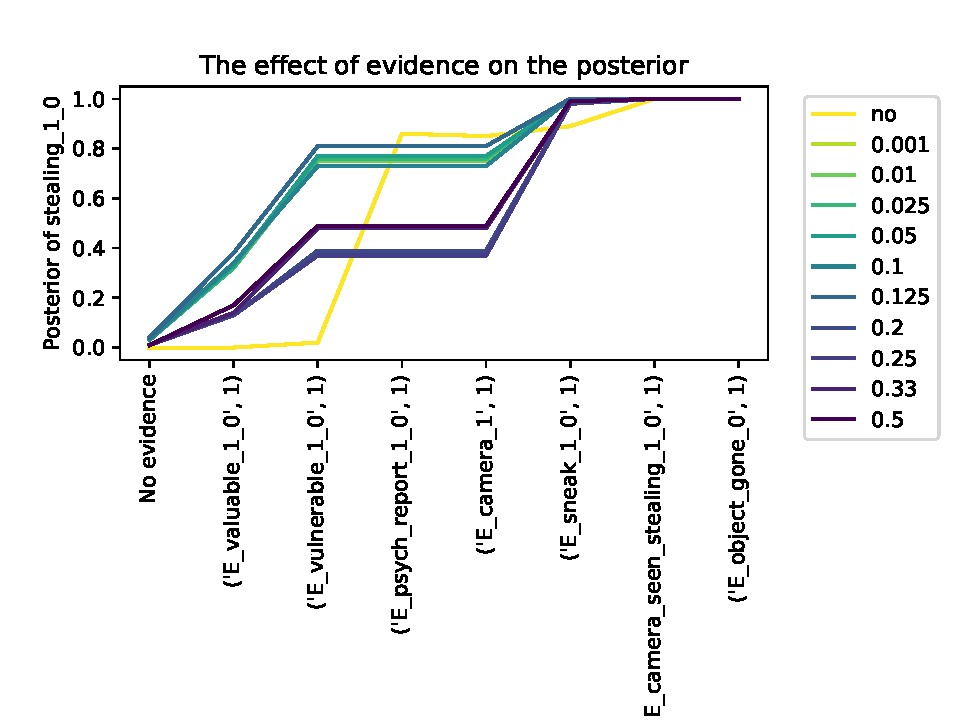
\includegraphics[width=0.9\linewidth]{../experiments/GroteMarkt/plots/posterior_GroteMarkt.pdf}
\caption{ Progression of evidence resulting in changing the posterior}
\label{post}
\end{subfigure}
\end{center}
\caption{Loss of precision in networks.}
\label{pLoss}
\end{figure}

We see again that the networks hold up well against loss of precision (Figure~\ref{pLoss}), which is promising for human builders, as long as they do not assign 1 and 0 but instead $1 - \epsilon$ and $\epsilon$.

\end{enumerate}

\subsection{Structural}

\begin{enumerate}
\item \textbf{The BN represents all events of the scenario}
No irrelevant events are in the network. There are some connections between nodes that seem irrelevant or overspecified, though.

\item \textbf{The BN has temporal ordering of the hypothesis nodes}
Due to the ordering as presented to the K2 algorithm, we see that most of the hypotheses nodes from the main scenario are ordered temporally. The node `object\_dropped\_accidentally\_0' is the one exception. This node represents the alternative scenario where the thief does not steal, but the victim agent drops their object by accident. When the two scenarios are merged when the ordering is presented to the K2 algorithm, the second scenario is added after the first scenario, but before the evidence, because the second scenario occurs less frequently. It is correct that the node is connected to the `motive\_1\_0'  and `stealing\_1\_0' nodes, because the thief cannot have a motive or steal an object of the victim if the victim does not possess the object anymore. Ideally, we would want this node to have no parents. That this does not happen is a flaw in the naive calculation of the temporal ordering - we should not just look at ordering, but at the time-step of the event instead to produce correct temporal ordering of merged scenarios.


\item \textbf{The BN follows the evidence-idiom}
Every piece of evidence has at least one hypothesis node as a parent, and no piece of evidence is the parent of a hypothesis node. The network satisfies this constraint, although not every hypothesis node has evidence applied to it.

\item \textbf{The BN represents multiple alternative scenarios}
(todo) We see that the conflicting scenarios are reflected in the BN.

\end{enumerate}

\subsection{Predictive}
\begin{enumerate}
\item \textbf{The BN only predicts high probability of the output node given relevant evidence truth values}

\begin{figure}[htbp]
\begin{center}
\begin{subfigure}{.66\textwidth}
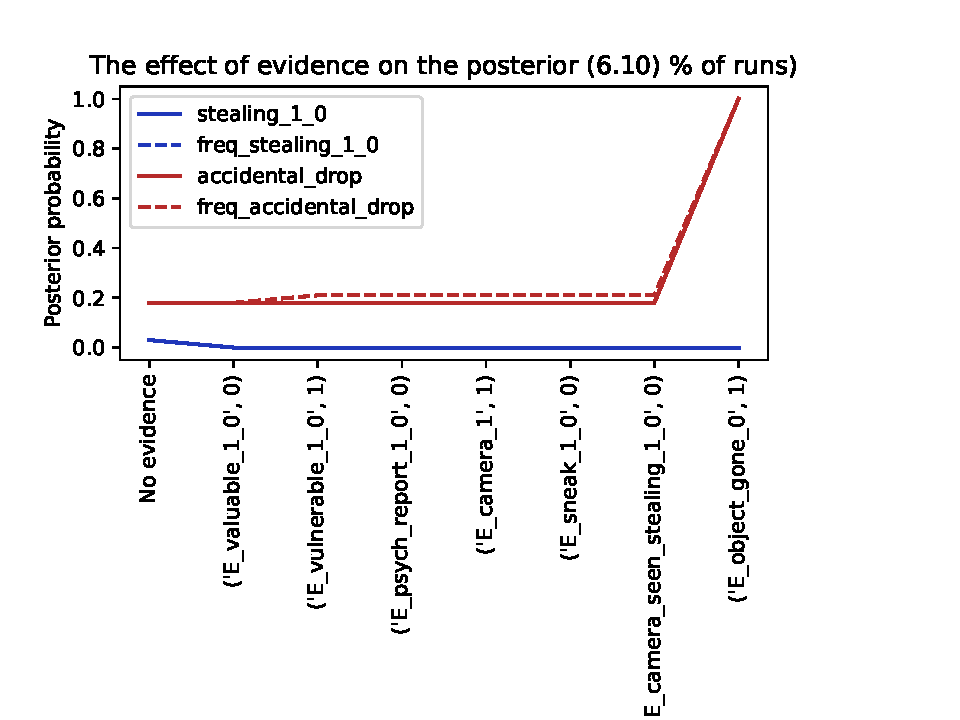
\includegraphics[width=\linewidth]{../experiments/GroteMarkt/plots/evidence_progress_GroteMarkt_1.pdf}
\caption{}
\label{default}
\end{subfigure}%
\begin{subfigure}{.66\textwidth}
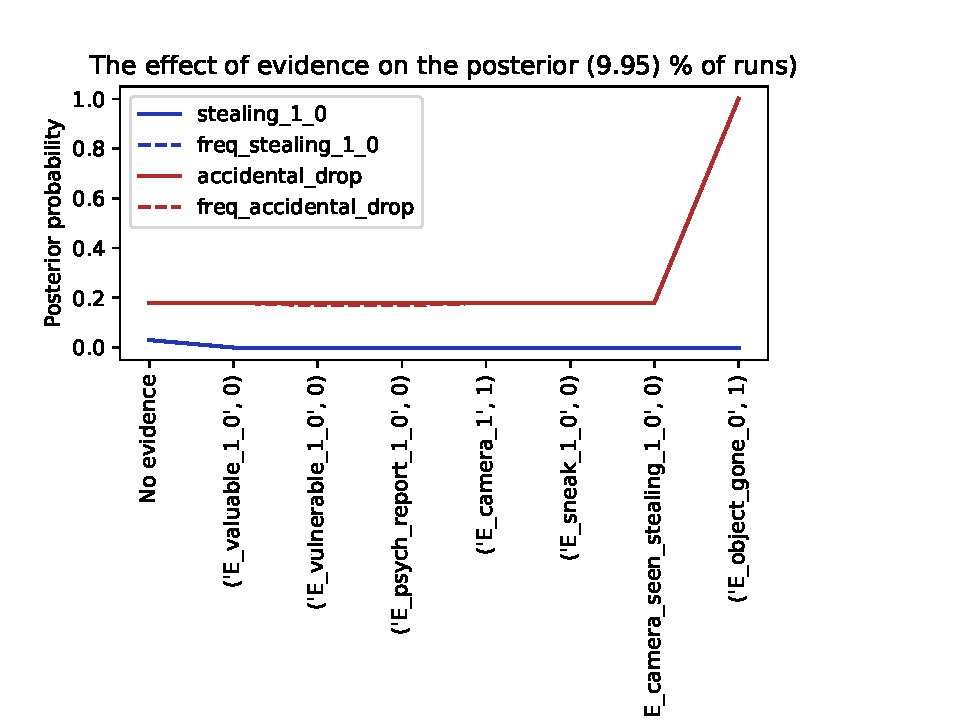
\includegraphics[width=\linewidth]{../experiments/GroteMarkt/plots/evidence_progress_GroteMarkt_2.pdf}
\caption{}
\label{default}
\end{subfigure}
\begin{subfigure}{.66\textwidth}
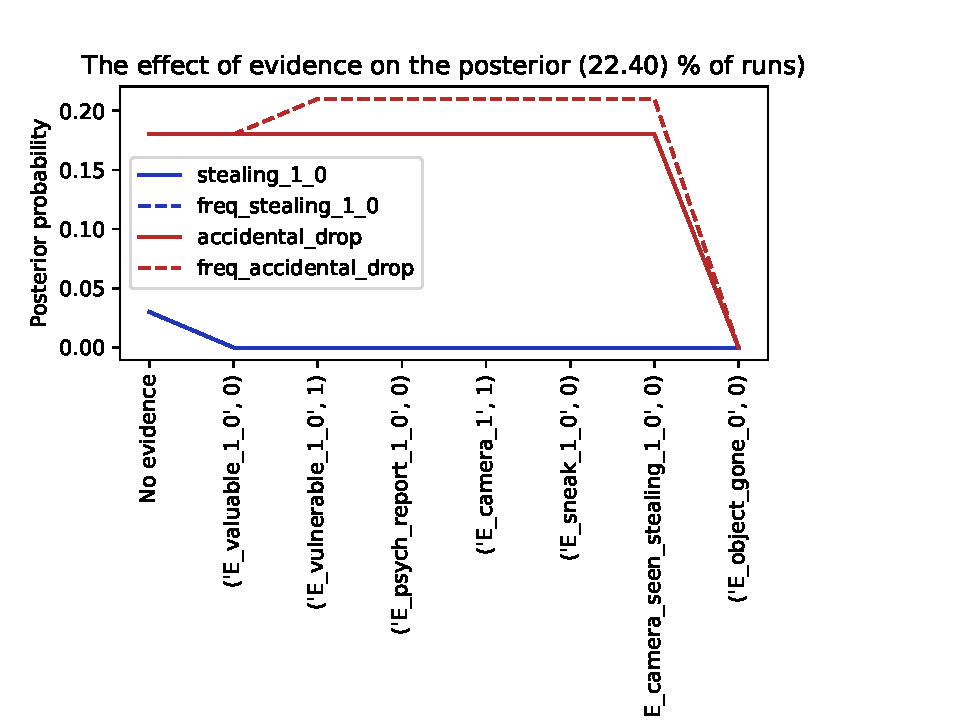
\includegraphics[width=\linewidth]{../experiments/GroteMarkt/plots/evidence_progress_GroteMarkt_3.pdf}
\caption{}
\label{default}
\end{subfigure}%
\begin{subfigure}{.66\textwidth}
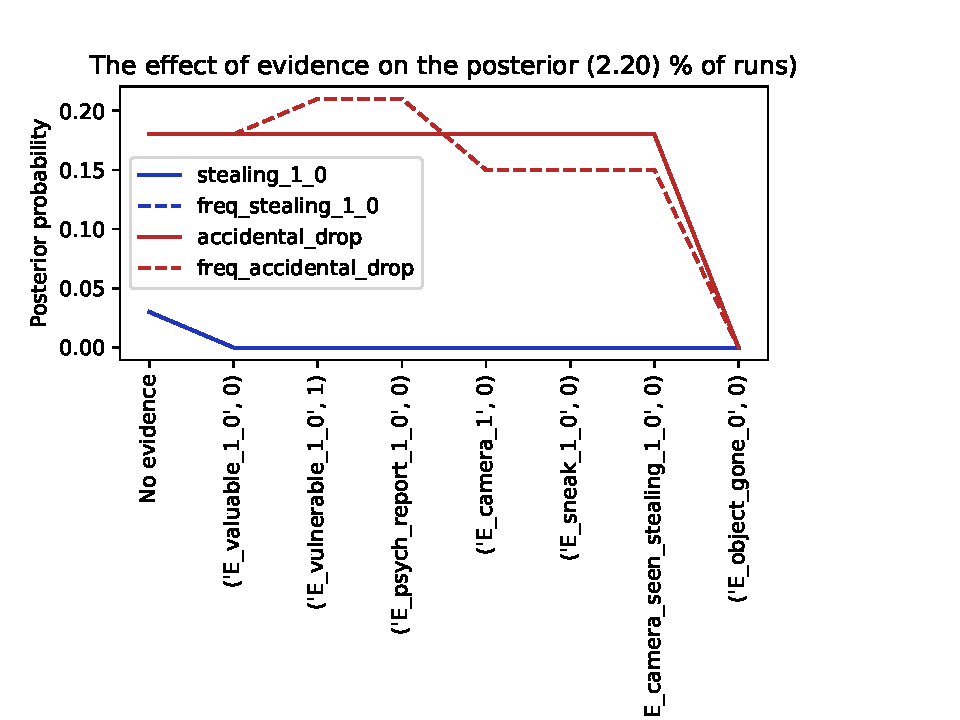
\includegraphics[width=\linewidth]{../experiments/GroteMarkt/plots/evidence_progress_GroteMarkt_4.pdf}
\caption{}
\label{default}
\end{subfigure}
\begin{subfigure}{.66\textwidth}
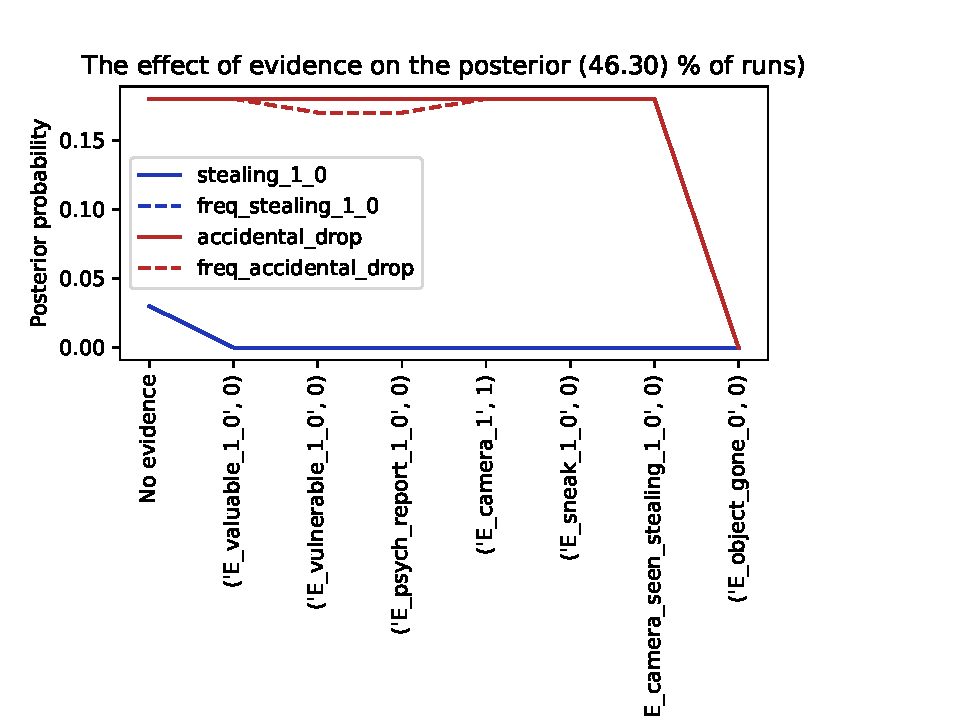
\includegraphics[width=\linewidth]{../experiments/GroteMarkt/plots/evidence_progress_GroteMarkt_5.pdf}
\caption{}
\label{default}
\end{subfigure}
\caption{Effect of evidence on posterior.}
\label{malthus}
\end{center}
\end{figure}

We see here that the posterior probability of the `stealing\_1\_0' node reflects exculpatory evidence well - as soon as we find evidence that would make it impossible for the agent to have stolen (such as not finding the other agent vulnerable, or the object valuable), the posterior for stealing immediately turns to 0. 

However, if we look at the progression of evidence in 4.4(a), where all the evidence is true, we see a posterior $>0.9$ for the `stealing\_1\_0' node as soon as we entered that the agent has a motive (`E\_psych\_report'). Depending on a given guilt threshold, this might be enough to convict. But this is very weak evidence in real life - just because the agent might have a motive, does not mean that it is going to steal. We see a small increase in the posterior when `E\_camera\_seen\_stealing\_1\_0' is set to true, when this should really be the strongest piece of evidence in the entire set. This shows that if we have access to the private knowledge of the agent (its intention to steal), we can make good predictions.

\item \textbf{We can know when the BN predicts the wrong outcome}
(todo)

\end{enumerate}

\section{Discussion}

We have shown in this chapter that we can generate satisfactory Bayesian Networks from simple agent-simulations with non-trivial environments. These networks can be used to reason towards a conclusion about a posterior probability, given a set of evidence. The network is accurate and is robust under imprecision. However, there are too many arcs in the network, and it is unclear how we should elicit the correct probabilities.

\subsection{Limitations of the simulation.}
This simulation should be seen as a preliminary for further research, as it is lacking in several aspects: the environment is still too simple, the agent-behaviour is too static, and there are only two agents in the simulation. These are the same weaknesses as identified in \citep{Zhu2021}. Expanding the simulation to include or improve these aspects is useful for future research.

The non-trivial environment is still not reflecting the non-trivialness of real environments. The environment of a city offers different affordances to different people, but here the map is shared by all agents. Additionally, shops and buildings can actually be entered.

There is a lack of dynamic behaviour in the agents. They can move around and decide to steal from someone, but they do so based on simple factors. This does not meaningfully reflect the real dynamics of street crime - for example, the vulnerable agent walks around with their valuable object in plain sight, why would they do that if they know that there are thieves on the loose?

One of the purposes of modelling a `real' location is to model the people within that real location. There are many people around on the Grote Markt in real life, modelling just two of them (and not modelling interactions with the crowd) is sufficient to show that automated Bayesian Networks might work in this situation. However, situations where Bayesian Networks might rely on statistical data from real samples (that might be taken from real locations, like the Island Prior), are not modelled in this simulation. 



\subsection{Problems}
\begin{enumerate}


\item \textbf{Does the BN not depend on private knowledge?}

We can think about the process of a criminal investigation and a trial as a systemic way
of gathering, sharing and finally agreeing on knowledge. Initially, only the criminal will
know the entire story, victims know parts of it, and the police and judges know even less.
An ideal trial results in common knowledge of the entire situation.

Of course, it is not in the interest of everyone to freely share their private knowledge all
the time. Police might not want to talk about the limitations of their evidence (or their
ways of procuring it), witnesses and victims might not want to talk due to incrimination,
shame, or relationships to the people involved. Suspects might not want to freely share
their murder plans (obviously). There is an abundance of private knowledge.

The Bayesian Network generated up till now, have not taken this into consideration. We
have the full set of nodes - even nodes that a realistic investigation cannot be sure about,
like the internal considerations of the criminal agent (like the its assessment of the victim or its tendency to steal). If we were real investigators, we cannot actually know this behaviour and hence cannot model
it in our network before the agent admits to the behaviour in court.

This would imply that we can only create Bayesian Networks after the fact: only when the
court case is over, and all the facts and their probabilities have been established, can we
start building them. Otherwise, we risk missing out on essential psychological or internal
information. This would not be ideal. This leads us to ask the question: do our networks
still work if we lose information about the internal intentions of agents?

We created a second network, based on the first scenarios, only now without the private knowledge. This means that the random variables E\_vulnerable\_1\_0, E\_valuable\_1\_0 , E\_sneak\_1\_0 are removed from the list of total random variables that are passed to the K2 algorithm. The resulting network is shown in Figure~\ref{everything}.

\begin{figure}
\begin{center}
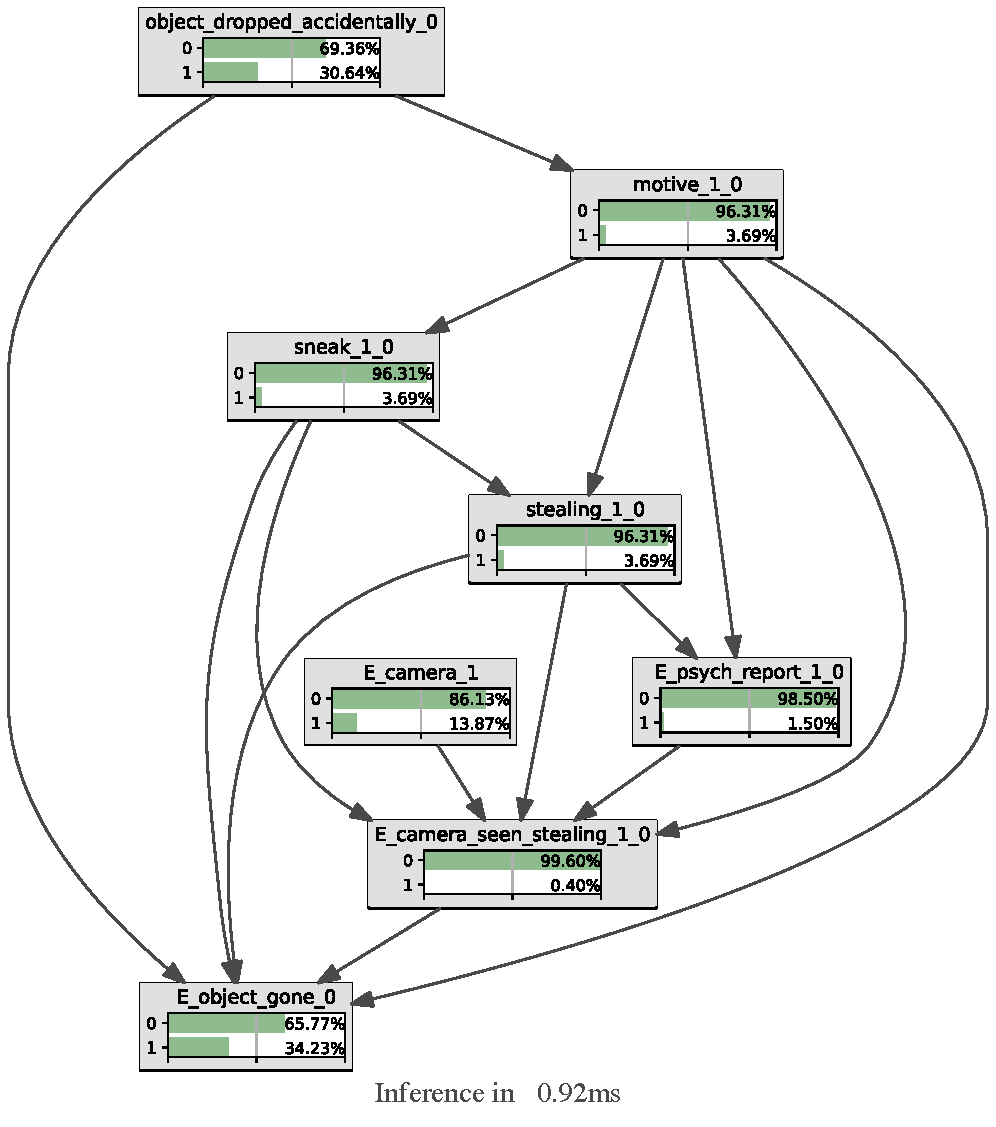
\includegraphics[width=1.2\linewidth]{../experiments/GroteMarktPrivate/bnImage/BNIMAGEGroteMarktPrivate.pdf}
\caption{Network of Grote Markt simulation.}
\label{everything}
\end{center}
\end{figure}

We find that this network has fewer nodes, the same temporal ordering as the original network, and might even be more easy to interpret due to these factors. If we look at the response of the output node to evidence valuations (Figure~\ref{all}), we see that the network results in the same pitfalls as the previous network: if all the evidence is true, we see that the most heavy evidence, which is the fact that the camera sees the agent steal, is 1, this does not affect the posterior belief in theft, which is high from the initial psychological report. This would not be strong evidence in a real-life court case.

\begin{figure}[htbp]
\begin{center}
\begin{subfigure}{.6\textwidth}
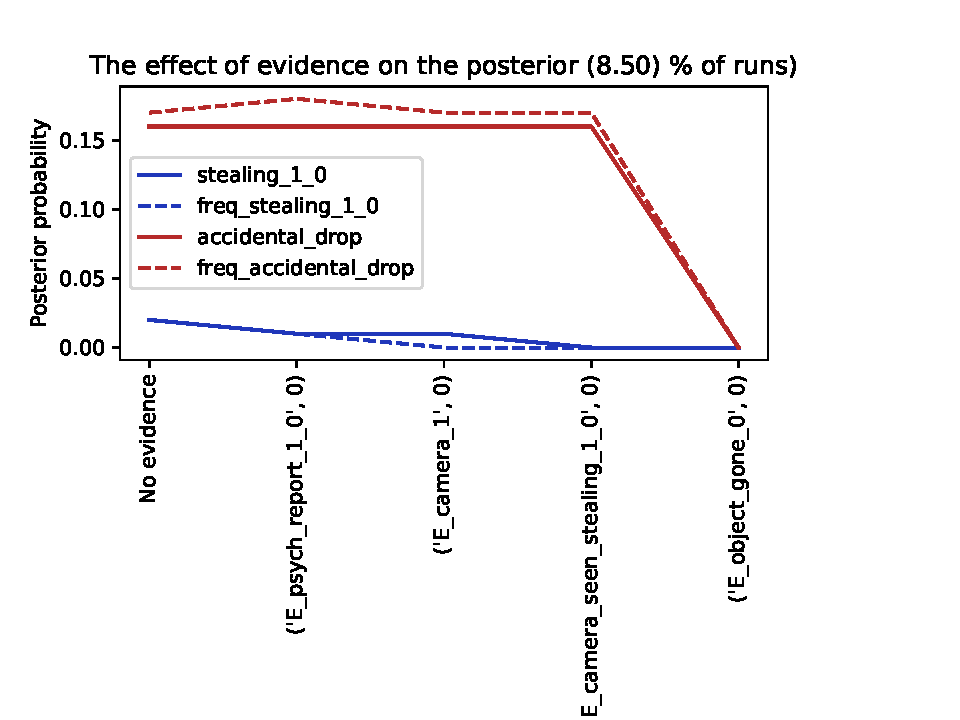
\includegraphics[width=\linewidth]{../experiments/GroteMarktPrivate/plots/evidence_progress_GroteMarktPrivate_4.pdf}
\caption{}
\label{default}
\end{subfigure}%
\begin{subfigure}{.6\textwidth}
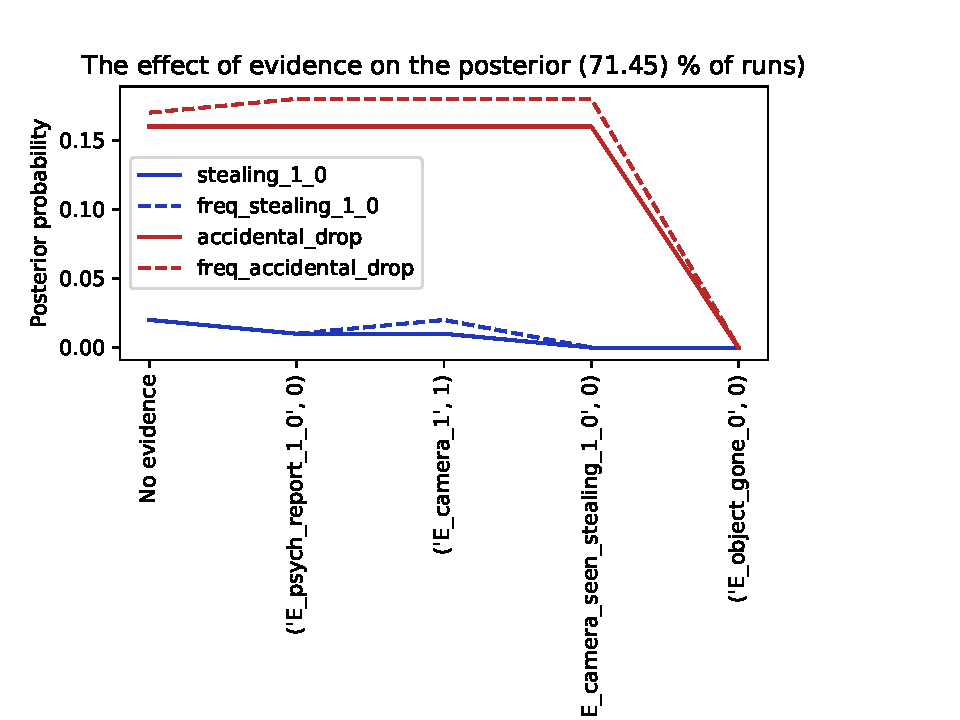
\includegraphics[width=\linewidth]{../experiments/GroteMarktPrivate/plots/evidence_progress_GroteMarktPrivate_1.pdf}
\caption{}
\label{default}
\end{subfigure}
\begin{subfigure}{.6\textwidth}
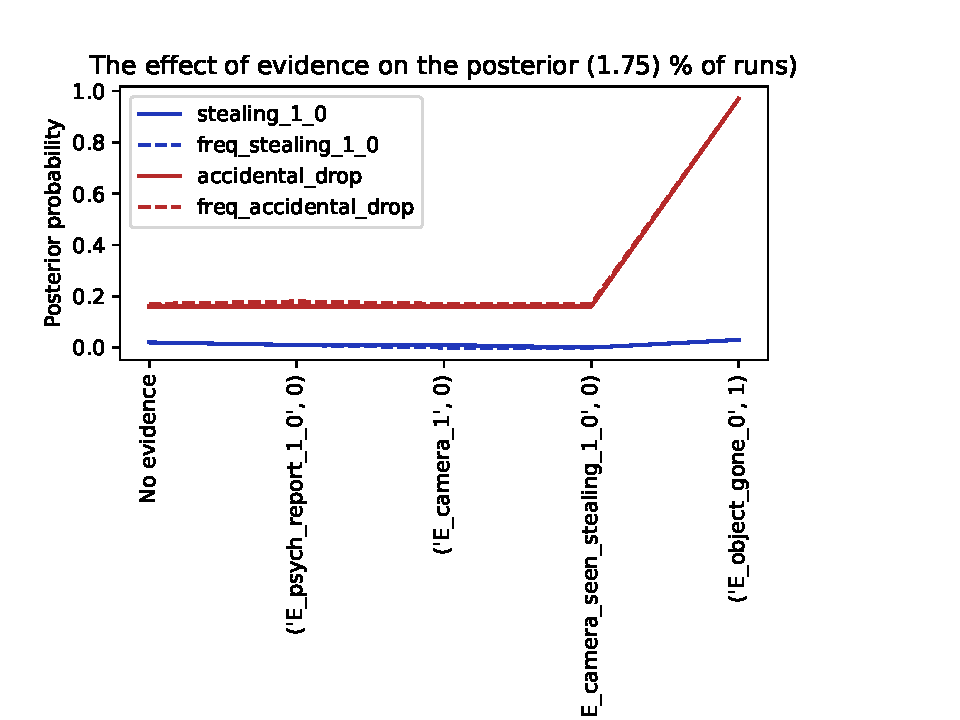
\includegraphics[width=\linewidth]{../experiments/GroteMarktPrivate/plots/evidence_progress_GroteMarktPrivate_3.pdf}
\caption{}
\label{default}
\end{subfigure}%
\begin{subfigure}{.6\textwidth}
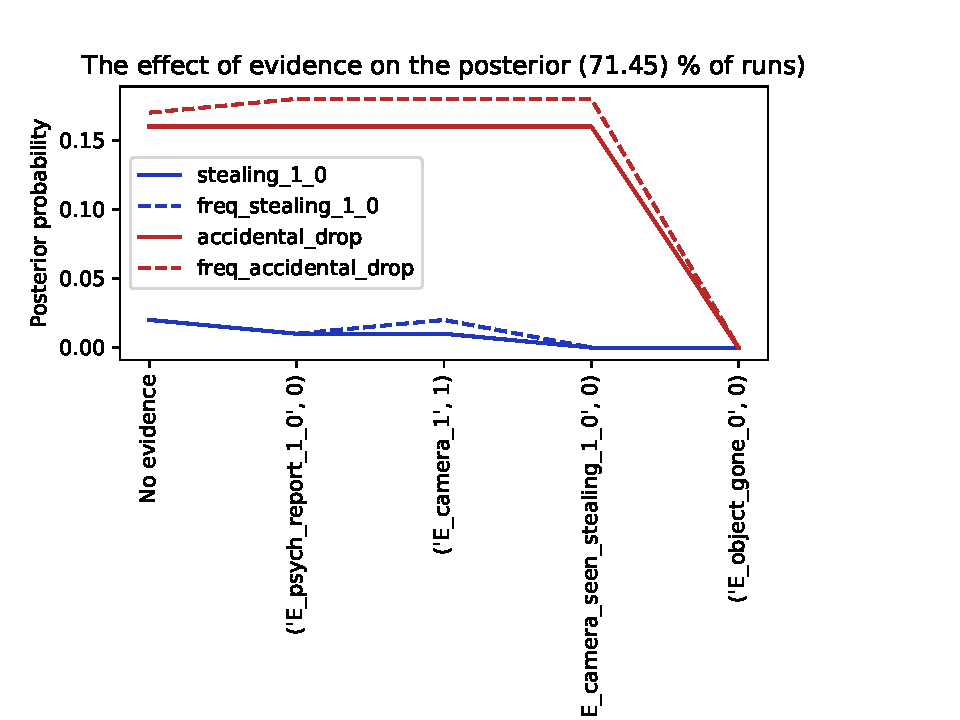
\includegraphics[width=\linewidth]{../experiments/GroteMarktPrivate/plots/evidence_progress_GroteMarktPrivate_1.pdf}
\caption{}
\label{default}
\end{subfigure}
\caption{Effect of evidence on posterior}
\label{all}
\end{center}
\end{figure}

\item \textbf{Could we apply this BN to a different location? }

We used one non-trivial environment to create this network. However, the underlying geometry of the simulation affects the probabilities that can be found in the simulation. We cannot just assume one prior probability for `seen\_1\_0', since the probability whether some agent sees the other, depends on the structure of the environment. We can show this by using the exact same agent behaviour, but placing the agents on a different map.

Instead of the Grote Markt, we selected 5 different parts of Groningen (Figure~\ref{maps}), converted them into maps according to the method, and then let the agents loose in them to rob each other.
\begin{figure}[htbp]
\begin{center}
\begin{subfigure}{.5\textwidth}
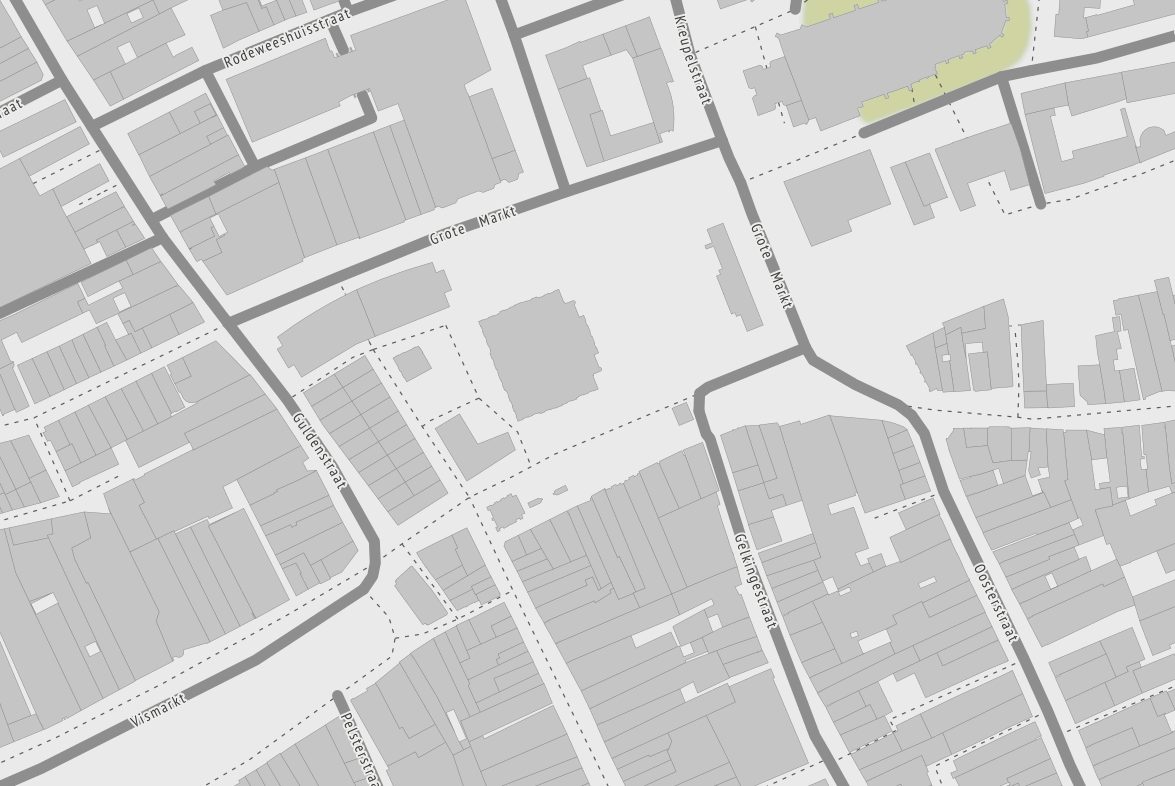
\includegraphics[width=0.8\linewidth]{../experiments/GroteMarktMaps/maps/groteMarkt.png}
\caption{Grote Markt.}
\end{subfigure}%
\begin{subfigure}{.5\textwidth}
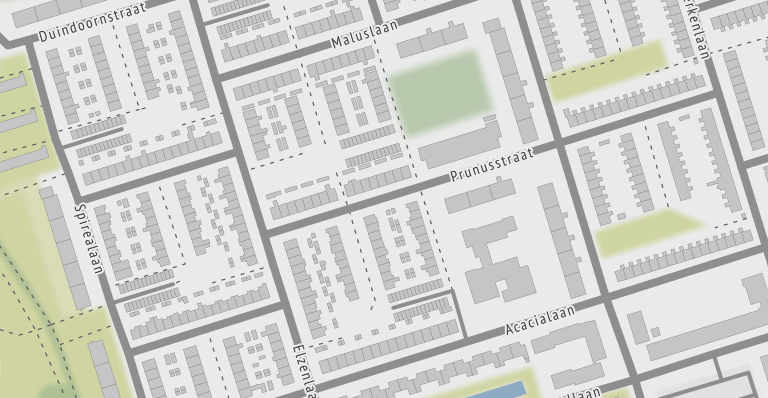
\includegraphics[width=0.8\linewidth]{../experiments/GroteMarktMaps/maps/Selwerd.png}
\caption{Selwerd.}
\end{subfigure}
\begin{subfigure}{.5\textwidth}
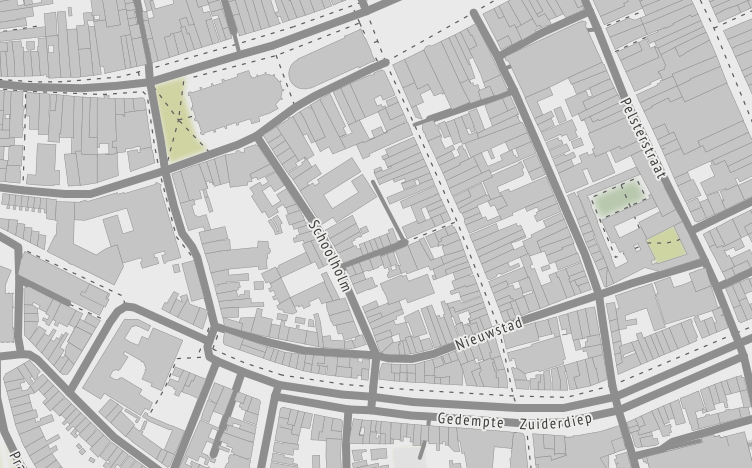
\includegraphics[width=0.8\linewidth]{../experiments/GroteMarktMaps/maps/zuidCentrum.png}
\caption{South-center}
\end{subfigure}%
\begin{subfigure}{.5\textwidth}
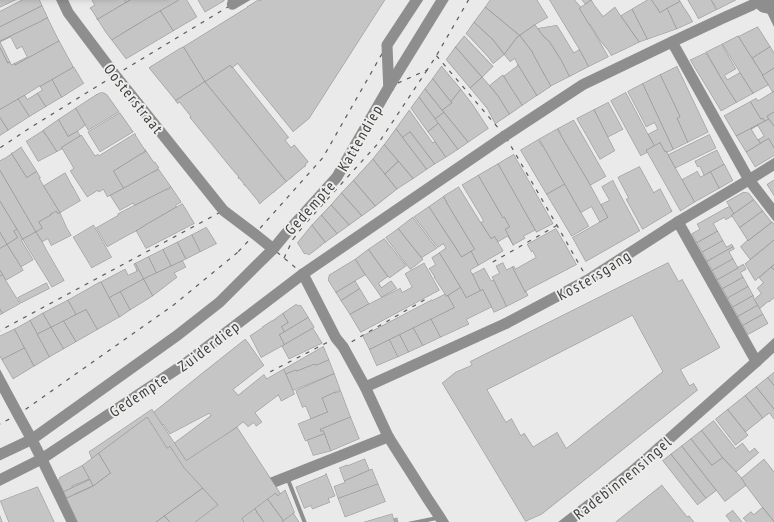
\includegraphics[width=0.8\linewidth]{../experiments/GroteMarktMaps/maps/kattediep.png}
\caption{Kattediep}
\end{subfigure}
\begin{subfigure}{.5\textwidth}
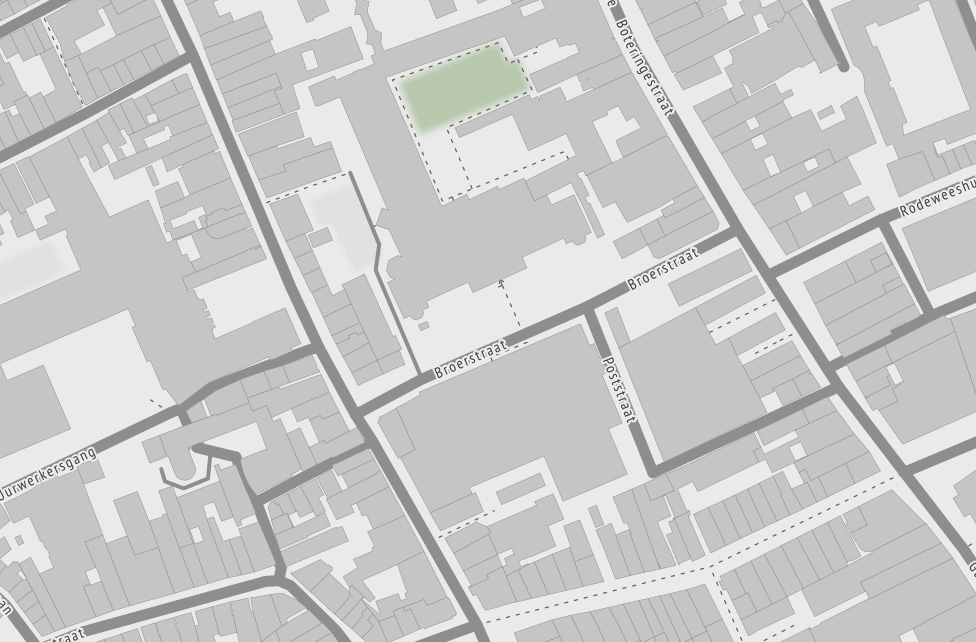
\includegraphics[width=0.8\linewidth]{../experiments/GroteMarktMaps/maps/academy.png}
\caption{Street with the academy building}
\end{subfigure}%
\begin{subfigure}{.5\textwidth}

\includegraphics[width=0.8\linewidth]{../experiments/GroteMarktMaps/maps/wall.png}
\caption{Not Groningen, just a wall}
\end{subfigure}
\caption{Maps.}
\label{maps}
\end{center}
\end{figure}


We look at the difference in the cpt tables for `seen\_1\_0', which represents the event that agent 1 (the thief), sees agent 0 (Table~\ref{mapstab}). If we did not need to condition on underlying geometry of the simulation, we would expect that this probability of `seen\_1\_0' would be the same, regardless of map. However, we find that the probability of the thief seeing the potential victim, depends on the underlying map. 

This means that we actually cannot speak of just one `global' probability for `seen\_1\_0'. The probability of the thief seeing the victim depends on a variable that is not included in the Bayesian Network: the map. Instead of a `global' probability for `seen\_1\_0', that applies to all maps, we can only speak of the probability of the agent seeing the victim as conditioned on a specific map. 

Implications of this is that we need to condition explicitly on maps for our networks to work, because it does meaningfully change the probabilities that we find. Additionally, there's no way to predict how the map that we're using affects the probability of `seen\_1\_0', this probability emerges from the interaction of the agents with the map. This has implications for the real world, because it means that we can't depend on some generic ``probability of getting robbed'', we need to condition on spatial conditions, and background world assumptions.

\begin{table}[htbp]
\begin{tabular}{llll}
map &  cpt of `seen\_1\_0' True \\
\hline
selwerd&  0.471\\
academy & .951\\
groteMarkt & 0.534\\
kattediep &0.534\\
wall &  0.512\\
zuidCentrum & 0.509\\
\end{tabular}
\caption{Difference in cpt depending only on difference in underlying map, no further difference in agent behaviour!}
\label{mapstab}
\end{table}



\item \textbf{Identity and guilt?}
We have avoided the problem of identity in this network, because we only have two agents, and one of the agents is always the thief, the other the victim. As soon as we create a more plausible simulation of crime, where everyone could, in principle, rob everyone, given the right incentives, we would need a different kind of reporter. Even if we created the same simulation, but now the victim agent might also be able to rob the thief-agent, we would need twice the amount of nodes (we need `stealing\_0\_1', and the rest as well). Three agents that can each rob each other, and we have 6 times as many nodes, resulting in for $n$ agents, $n(n-1)$ number of nodes if we use the same structure. This is very implausible due to complexity constraints. However, generalising the nodes (so using `stealing', instead of `stealing\_0\_1') means that we have to represent the identity of the suspect in some other way. It is unclear how that is to be done.


\end{enumerate}


\subsection{Possible Legal Interpretations.}

As we found in the network in the previous chapter, the problem of operationalisation continues to haunt us. The simulation has very clear operationalisation, as represented by the always-correct reporters. However, it is unclear what shape these reporters should take outside of our simulation. Lawyers and judges would have to ask themselves the following questions, to be applied to every node:

\begin{itemize}
\item \textbf{By what method can we find out whether this event happened or not?}

This question can be answered relatively easily for evidence nodes. For instance, we would know that `E\_camera\_1' would be true in real life, if we saw agent 1 on a relevant camera. For our psychological report, we would know that this event did not happen if the psychiatrist decided that the victim did not fit the suspect's profile.

However, this becomes very complex for hypothesis nodes. How would you find out of `stealing\_1\_0' is true in real life? In our simulation, we just set the event to 1 if it happened. In real life, how would you operationalise this? It is unclear. Should we decide that `stealing\_1\_0' is true if the victim says that their object was stolen? That's perhaps a part of an operationalisation, but it is not a completely valid one, since we know that people can lie about their stuff being stolen. If we say, the victim should say that their object was stolen, and we should find the object on the thief, we are still in trouble if the thief decides to sell the object before they can be apprehended. What would be the method to find out that the state of the real world is such that you could say that `stealing\_1\_0' is true, or false?

 In the real world, we do not need an operationalisation for these kinds of facts, because we all `sort of know what we mean'. However, in Bayesian Networks we need an operationalisation, because Bayesian Networks and random variables are mathematical objects, and need to map events to truth values. This cannot be done without operationalisation.

\item \textbf{If we have a method, how do we decide which events we want to include in our frequency calculation?}

This is the problem of the reference class. To take the example of camera, if we include all cameras in the inner city, the probability that the thief would be seen is great, and hence would not be very relevant to proving the thief's guilt. However, if we decide that we will only use cameras that were on the victim's trajectory, we have limited the amount of cameras, and the probability of the thief showing up on one of these `coincidentally' is lower, hence it would be a stronger piece of evidence if we found that it was true (and more exculpatory if we found that it was false). 

Even though the reference class is a fundamental problem, as long as every legal participant is aware of it, and can argue about why some reference class is better than another class, or decides on the appropriate classes together, this should not be a limiting factor for the Bayesian Network in itself. However, it requires a great deal of work that would not be done if Bayesian Networks were not used, and it is unsure if it would actually result in better outcomes.

\end{itemize}

These essential questions should come before talking about Bayesian Network accuracy, precision or structure, especially if these networks are to be used for practical applications.



